%% -*- mode: latex; mode:flyspell -*-
\documentclass[svgnames,x11names]{beamer}

\usepackage[british]{babel}

\usepackage{minted,tikz,tcolorbox,calc,siunitx}
\usetikzlibrary{chains,positioning,calc,shadows,arrows,matrix}
\usetikzlibrary{shapes.geometric,shapes.symbols}
\usetikzlibrary{circuits,circuits.logic,circuits.logic.IEC}

\usepackage{pgfplots}
\usepackage{booktabs,inconsolata}

\usepackage{tikz-timing}
\usetikztiminglibrary{either}
\usetikztiminglibrary{counters}
\usetikztiminglibrary{beamer}

\title{Polling vs Interrupts}
\subtitle{CM0506 -- Small Embedded Systems}
\date{Lecture 5}
\author{Dr Alun Moon}
\institute{Department of Computer and Information Science}

\definecolor{NUblue}{RGB}{62,141,165}
\definecolor{NUbluedark}{RGB}{40,119,143}

\usetheme{CambridgeUS}

\usecolortheme{crane}
\setbeamercolor*{palette primary}{use=structure,fg=white,bg=NUblue}
\setbeamercolor*{palette quaternary}{fg=white,bg=NUbluedark}
\setbeamercolor{section in head/foot}{fg=white,bg=NUbluedark}
\setbeamercolor{subsection in head/foot}{fg=white,bg=NUblue}
\setbeamercolor{frametitle}{fg=NUbluedark!150,bg=NUblue!40}
\setbeamercolor{title in head/foot}{fg=white,bg=NUblue}
\setbeamercolor{author in head/foot}{fg=white, bg=NUbluedark}
\setbeamercolor{date in head/foot}{fg=white, bg=NUblue!60}
\setbeamercolor{title}{fg=NUbluedark!150,bg=NUblue!30}
\setbeamercolor{date}{fg=NUbluedark!150}
\setbeamercolor{block title}{fg=white,bg=NUblue}

\usepackage[T1]{fontenc}
\usepackage[utf8]{inputenc}

\begin{document}

\frame\maketitle

\begin{frame}[fragile]{Polling}{Periodically checking devices}
  \begin{block}{}
    \begin{minted}{c}
      while(1) {
        wait(200);
        if (buttonPressedAndReleased(&pin[JLEFT])) {
          flashing[LED1] = !flashing[LED1];
        }
        if (buttonPressedAndReleased(&pin[JDOWN])) {
          flashing[LED2] = !flashing[LED2];
        }
      }
    \end{minted}
  \end{block}
  \begin{itemize}
  \item Check for condition of device
  \item if data is available
  \item read the device or do something
  \item repeat
  \end{itemize}
\end{frame}

\begin{frame}[fragile]{Polling}
  \begin{block}{}
    \begin{minted}{c}
      bool buttonPressedAndReleased(gpioPin_t *pin) {
	bool result = false;
	if (gpioPinVal(pin) == 0) {
		while (gpioPinVal(pin) == 0) {
			/* skip */
		}
		result = true;
	}
	return result;
      }
    \end{minted}
  \end{block}
  \begin{itemize}
  \item Software has to keep checking status of device
  \end{itemize}
\end{frame}

\begin{frame}[fragile]{Polling}
  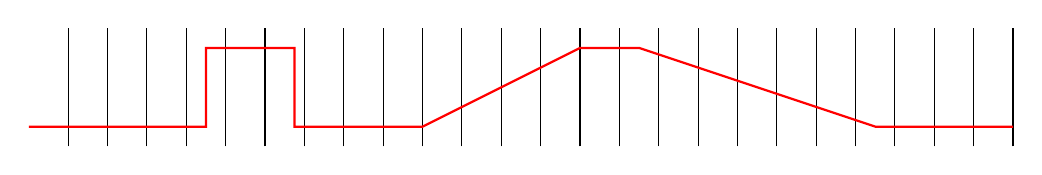
\begin{tikzpicture}[xscale=0.5]
    \foreach \x in {1,...,25}
      \draw (\x,-0.25) -- (\x,1.25);
      \draw[red,thick] (0,0) -- (4.5,0) -- (4.5,1) -- (6.75,1) -- (6.75,0) --
       (10,0) -- (14,1) -- (15.5,1) -- (21.5,0) -- (25,0);
  \end{tikzpicture}
  \begin{description}
  \item[Level sensitive] Test value of input at sample points 
    \begin{itemize}
    \item what is 1 or 0
    \end{itemize}
  \item[Edge sensitive] Test for changes in level
    \begin{description}
    \item[Rising Edge] level goes from low (0) to high (1)
    \item[Falling Edge] level goes from high (1) to low (0)
    \end{description}
  \end{description}
  \begin{alertblock}{}
    What happens if the signal changes between sample points?
  \end{alertblock}
\end{frame}

\begin{frame}{Polling}
  \begin{itemize}
  \item Also called \alert{Synchronous} I/O
  \item For many applications:  most polled samples will mean ``nothing happening here''
  \item Considerable time may be spent executing code for long
    intervals when no input is available to work on 
  \item This may be OK if there is nothing else to do \ldots but \ldots
  \end{itemize}
\end{frame}

\begin{frame}{Polling more than one input}
  \begin{itemize}[<+->]
  \item What if there are many inputs which have to be sampled?
  \item The application will have to scan each input and react if the
    input is active (interesting)
  \item Manageable under some circumstances
  \item It may become difficult if the number of inputs is large and
    other tasks require processing.
  \item System may be slow to react to inputs
    \begin{itemize}
    \item you have to wait until the next sample for that input
    \end{itemize}

  \end{itemize}
\end{frame}

\begin{frame}{Interrupts}
  \begin{itemize}
  \item A peripheral device may be connected to the CPU by an
    \alert{Interrupt request} line
    \begin{itemize}
    \item Identified by a number
    \item May by \emph{on chip} devices, timers, communications
    \item May be \emph{external} IO ports, dedicated interrupt pins
    \end{itemize}
  \item The \alert{Interrupt vector table} has a corresponding list of
    addresses for interrupt handler routines
    \begin{itemize}
    \item an array of addresses
    \end{itemize}
  \end{itemize}

  \begin{block}{Actions on an interrupt}
    \begin{enumerate}
    \item CPU finishes current instruction (machine level/assembler)
    \item saves a snapshot of its state
    \item looks up the address of the interrupt handler in the vector
      table
    \item branches to this address
    \item on exiting the interrupt handler, restores the saved state
    \end{enumerate}
  \end{block}
\end{frame}

\begin{frame}{Interrupts}
  \begin{itemize}
  \item \alert{Asynchronous} deviation of execution path
  \item can occur between \emph{any two} machine instructions
  \item beware side effects of interrupt handler.
  \end{itemize}

  \begin{block}{Interrupt Latency}
  \begin{itemize}
  \item The Delay between the event occuring and the execution of the
    corresponding handler
  \item Many factors can influence:
    \begin{itemize}
    \item Completion of current instruction
    \item Fetch of interrupt vector
    \item Completion of any higher priority interrupts
    \end{itemize}
  \end{itemize}
\end{block}
\end{frame}
\begin{frame}
  \frametitle{Interrupts and Complexity}
  \begin{itemize}
  \item Interrupt based solutions can be \alert{very} difficult to
    debug
  \item Hard to demonstrate correctness
  \item Interrupts can interfere in unexpected ways -- especially if
    shared resources are involved
  \end{itemize}
\end{frame}
\part{Code structure and hints}
\frame\partpage

\begin{frame}{Interrupt handler}
  \begin{itemize}
  \item \alert{No} parameters passed or returned
  \item need to use \alert{globals} to pass information between
    interrupts and other parts of code
  \item Usually some hardware related \emph{boiler-plate} code to
    manage flags.
  \end{itemize}
\end{frame}

\begin{frame}[fragile]{Split hardware interrupt related and
    application related}
  \begin{exampleblock}{}
\begin{minted}{c}
void (*timer0_handler)(uint32_t match);
void TIMER0_IRQHandler(void)
{
	timer0_handler(LPC_TIM0->IR);
	LPC_TIM0->IR |= (1UL << 0);
}

\end{minted}
  \end{exampleblock}
  \begin{exampleblock}{}
\begin{minted}{c}
void flash(void)
{
	toggle_led(left_blue);
}
int main()
{
	initialise_timer0(ms,1000,flash)
}
\end{minted}
  \end{exampleblock}
  
\end{frame}

\begin{frame}
  \frametitle{Advantages}
  \begin{itemize}
  \item Separated interrupt specific code from application code
  \item Easy and hard bits to write and test
  \item Keeps application logic together in same file.
  \item Scope rules help avoid unwanted interactions
  \end{itemize}
\end{frame}


\begin{frame}[fragile]
  \begin{block}{scoping rules}
\begin{minted}{c}
static int flashing;
void flash(void)
{
	if( flashing ) toggle_led(left_blue);
}
int main()
{
	if( button_pressed() )
		flashing = 1;
	else
		flashing = 0;
}
\end{minted}
  \end{block}
\end{frame}

%%%% --------
\end{document}
%% Local Variables:
%% mode: reftex
%% mode: auto-fill
%% mode: flyspell
%% End:
